%\setcounter{chapter}{13} % "N" (14th letter, but latex first increments -> 14-1=13)
\chapter{Channel Estimation} \label{ch:channel}

In this chapter, we present a detailed analysis of the five proposed communication channels.
Metrics such as frequency response, $\gamma_{\text{ISI}}$, Power Delay Profile (PDP), and Bit Error Rate (BER) were utilized to characterize and compare their performance.
The varying nature of these channels introduces distinct impairments that complicate reliable transmission.

\section{Quantification of ISI}%
\label{sec:ISI Characterization}
\dirTeXtured{chapters/ISI/}

The phenomenon of Intersymbol Interference (ISI) arises from the time dispersion $T_p$ of the physical channel, which is formally defined by the interval $t_{inf} \le t \le t_{sup}$ where the impulse response $p(t)$ remains non-zero. As discussed in \textcite{ComunicacionesDigitales2012}, the discrete equivalent model $p[n]$ captures the interference between adjacent symbols. By normalizing the observation by the cursor $p[d]$, we decompose the signal at the decider input into three fundamental components:
\begin{figure}[!ht]
    \fcapside[\FBwidth]{%
        \captionsetup{parskip = .5\baselineskip plus 1pt}%
        \caption[Time Dispersion and Discrete Mapping]{%
            Impulse response $p(t)$ illustrating the relation between $T_p$ and the sampled coefficients $p[n]$ \autocite{Artes2012}.
        }%
        \label{fig:isi-dispersion}%
    }{%
        
\includegraphics[width=0.4\textwidth]{figures/chap3_channel/1.png}
    }
\end{figure}
\begin{equation} \label{eq:ISI_decomposition}
    \frac{q[n]}{p[d]} = A[n-d] + \sum_{k \neq d} \frac{p[k]}{p[d]} A[n-k] + \frac{z[n]}{p[d]} \eqend
\end{equation}
To evaluate the system's performance, we analyze the worst-case error bound using the triangle inequality:
\begin{align}
    \left| \frac{q[n]}{p[d]} - A[n-d] \right| &= \left| \sum_{k \neq d} \frac{p[k]}{p[d]} A[n-k] + \frac{z[n]}{p[d]} \right| \nonumber \\
    &\le |A|_{\text{max}} \underbrace{\sum_{k \neq d} \frac{|p[k]|}{|p[d]|}}_{D_{\text{peak}}} + \frac{|z[n]|}{|p[d]|} \label{eq:ISI_bound_derivation}
\end{align}
The relationship between the \emph{peak distortion} $D_{\text{peak}}$ and the constellation's \emph{robustness factor} $\eta$ determines the total ISI level $\gamma_{\text{ISI}}$. These parameters are defined as:
\begin{equation} \label{eq:ISI_metrics}
    D_{\text{peak}} \doteq \sum_{k \neq d} \frac{|p[k]|}{|p[d]|} \eqcomma \qquad \eta \doteq \frac{d_{\text{min}}/2}{|A|_{\text{max}}} \eqcomma \qquad \gamma_{\text{ISI}} \doteq \frac{D_{\text{peak}}}{\eta} \eqend
\end{equation}
By substituting \eqref{eq:ISI_metrics} into the error bound \eqref{eq:ISI_bound_derivation}, we obtain the final condition for error-free transmission in noiseless scenarios ($z[n]=0$):
\begin{equation} \label{eq:final_ISI_bound}
    \left| \frac{q[n]}{p[d]} - A[n-d] \right| \le \gamma_{\text{ISI}} \left( \frac{d_{\text{min}}}{2} \right) + \frac{|z[n]|}{|p[d]|} \eqend
\end{equation}
\begin{remark}[Eye Diagram Closure]
    If $\gamma_{\text{ISI}} < 1$, the eye diagram remains open, meaning the distortion is smaller than the decision distance $d_{\text{min}}/2$. Conversely, when $\gamma_{\text{ISI}} > 1$, the interference alone causes errors, regardless of the Signal-to-Noise Ratio (SNR).
\end{remark}
\begin{Note}[Rate Dependency]
    The number of interfering samples $K = \lfloor T_p / T \rfloor$ increases as the transmission rate $R=1/T$ grows. Thus, a fixed dispersive channel may exhibit negligible ISI at low speeds but become unusable as $T$ decreases below $T_p$.
\end{Note}

\section{Methodology} \label{sec:Methodology}

To evaluate the channels, we employed a Least Squares (LS) estimation technique \autocite{Edfors1998}.
The LS algorithm derives the channel estimate from the training symbol located immediately after the preamble, representing a full OFDM symbol.
The channel frequency response, denoted as $\hat{H}[k]$, is obtained by dividing the received signal $Y[k]$ by the known pilot symbols $X[k]$ for each subcarrier $k$:
\begin{equation}
    \hat{H}_{\text{LS}}[k] = \frac{Y[k]}{X[k]}.
\end{equation}
When specific subcarriers are deactivated using a spectral mask, estimation is performed solely on the active frequencies.
By applying the Inverse Fast Fourier Transform (IFFT) to these frequency coefficients, we obtain the Channel Impulse Response (CIR).

\subsection{Practical MMSE Approximation} \label{sub:PracticalMMSE}

Observation of the CIR reveals that for most channels---particularly those exhibiting multipath propagation---the energy is concentrated in a finite duration.
The raw LS estimation, however, captures noise across the entire observation window, resulting in a \enquote{noisy} frequency response.
To mitigate this, we implemented a practical approximation of the Minimum Mean Square Error (MMSE) estimator.
This technique involves \enquote{windowing} the time-domain CIR: retaining the significant initial samples (taps) that represent the physical channel and zero-padding the rest.
Applying the FFT to this cleaned CIR yields a smoothed spectral estimate.
Mathematically, this approaches the theoretical MMSE solution and functions analogously to a low-order Moving Average process, significantly improving BER by rejecting noise outside the channel's delay spread.

\section{Channel 1: AWGN and Receiver Filtering} \label{sec:Channel1}

Channel 1 represents a classical Additive White Gaussian Noise (AWGN) scenario.
Ideally, an AWGN channel affects neither the phase nor the magnitude of the transmitted signal, implying that equalization might be unnecessary.
Examination of the impulse response confirms it approximates a delta function; however, the received signal is shaped by the receiver's front-end filter (typically an 8k band-pass filter).
Consequently, subcarriers at the band edges suffer varying degrees of attenuation compared to the center frequencies.

While LS equalization could invert this effect, it indiscriminately amplifies the noise.
The practical MMSE approach is superior here, as it models the filter's shape without enhancing the noise floor.
\Cref{fig:ch1_constellation_comparison} illustrates the resulting open eye pattern, confirming low Inter-Symbol Interference (ISI).

\begin{figure}[!ht]
    \centering
    \captionsetup{parskip = .5\baselineskip plus 1pt}
    \begin{tabular}{ccc}
        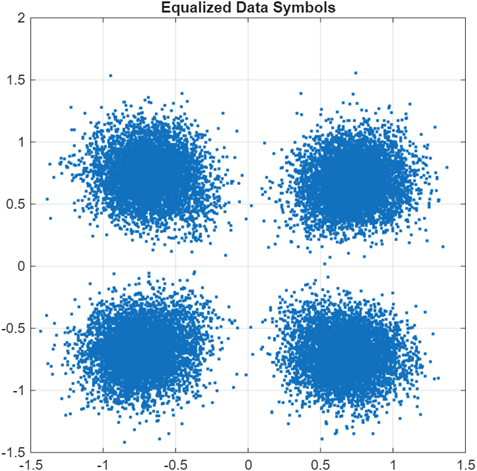
\includegraphics[width=0.3\textwidth]{figures/chap3_channel/c1_3.png} &
        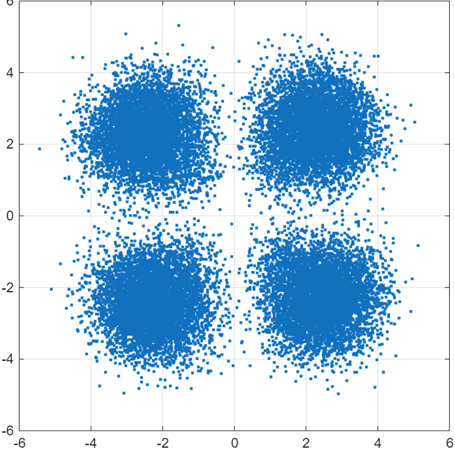
\includegraphics[width=0.3\textwidth]{figures/chap3_channel/c1_4.png} &
        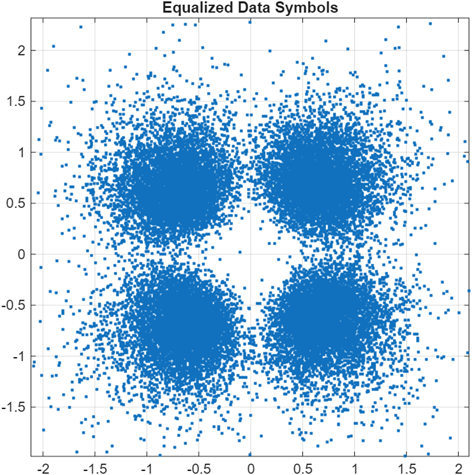
\includegraphics[width=0.3\textwidth]{figures/chap3_channel/c1_2.png} \\
        \small (a) MMSE Equalization & \small (b) LS Equalization & \small (c) No Equalization
    \end{tabular}
    \caption[Channel 1: Comparison of Equalization Techniques]{%
        Constellation comparison for Channel 1: (a) MMSE equalization provides optimal clustering; 
        (b) LS equalization shows higher noise sensitivity; 
        (c) Unequalized signal exhibiting an open eye pattern due to low ISI levels.
    }%
    \label{fig:ch1_constellation_comparison}%
\end{figure}

The impulse response and frequency magnitude are detailed in the appendix (see \Cref{fig:ch1_channel_estimation_summary}). The slight attenuation at the band edges is visible in the frequency response, which the MMSE estimator tracks smoothly.

\newpage

For Channel~1 (AWGN), the system achieves BER $<$ 1\% at about 3.5~dB SNR, both with and without FEC. As shown in Figure~\ref{fig:BERChannel1}, the coding gain from FEC becomes noticeable only at higher SNR values or for very low BER targets.

\begin{figure}[!ht]
    \fcapside[\FBwidth]{%
        \captionsetup{parskip = .5\baselineskip plus 1pt}%
        \caption[]{%
             Physical experimental setup showing the acoustic transmission environment.
        }%
        \label{fig:BERChannel1}%
    }{%
        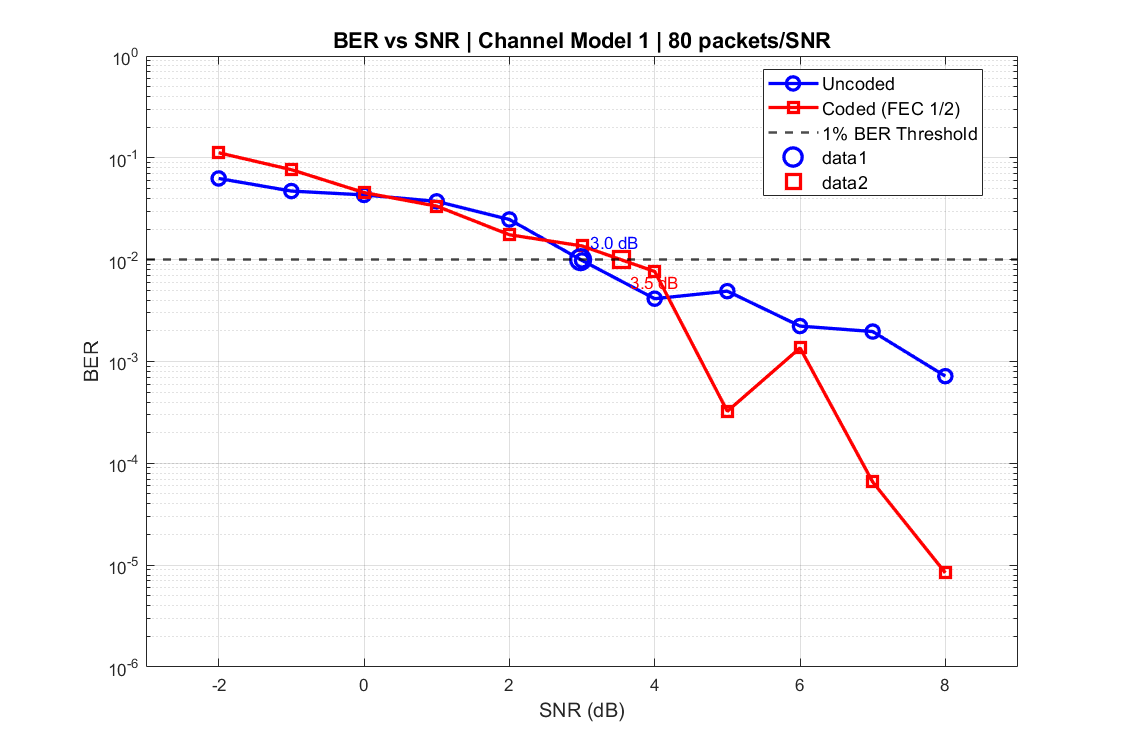
\includegraphics[width=0.70\textwidth]{figures/chap3_channel/BERChannel1.png}
    }
\end{figure}

\section{Channel 2: Phase Shift} \label{sec:Channel2}

Channel 2 shares the noise characteristics of Channel 1 but introduces a distinct phase shift.
Since the channel estimation is performed on a single training symbol at the start of the frame, time-varying phase drifts would only be visible if estimation were performed on a per-symbol basis.
However, in this static context, the constant phase rotation is evident.

Fortunately, the implemented synchronization system, which utilizes known QPSK pilots inserted into specific subcarriers of every data symbol, automatically corrects this phase offset.
Therefore, the performance and equalization strategies remain consistent with Channel 1. The effect of the equalization on the constellations is shown in \Cref{fig:ch2_constellations} in the appendix.

The channel estimation report (see \Cref{fig:ch2_report}) confirms a low ISI index, similar to the AWGN case.

\begin{figure}[!ht]
    \ffigbox[\FBwidth]{%
        \begin{tabular}{cc}
            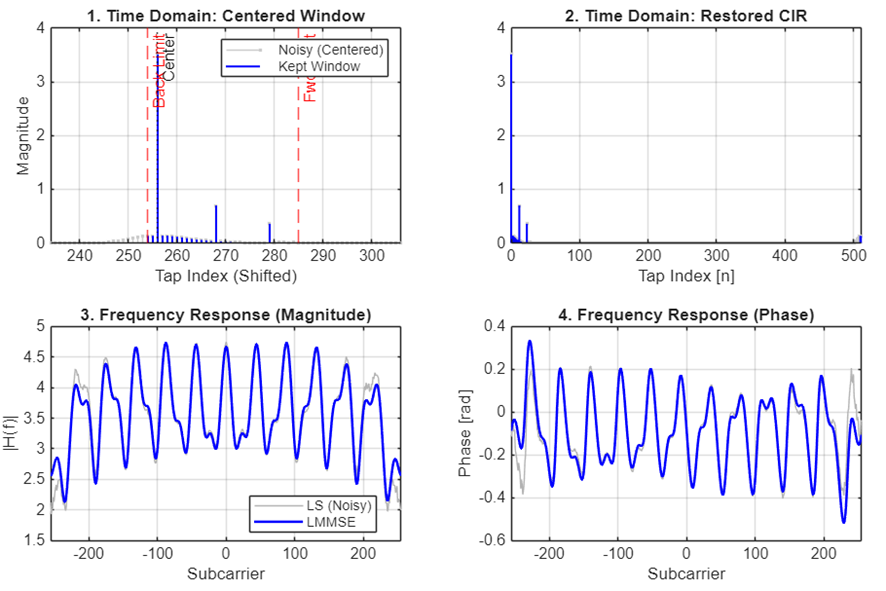
\includegraphics[width=0.67\textwidth]{figures/chap3_channel/c3_1.png} & 
            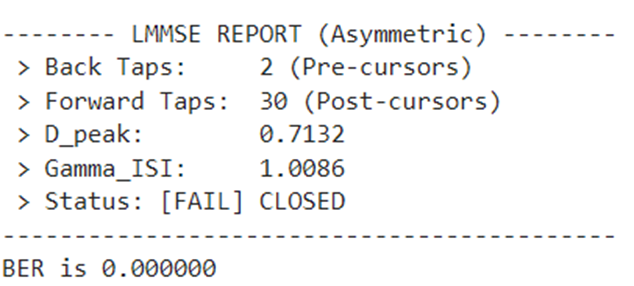
\includegraphics[width=0.27\textwidth]{figures/chap3_channel/c3_2.png} \\
        \end{tabular}
    }{%
        \caption[Channel Estimation and ISI Report]{%
            (Left) Time domain CIR windowing and Frequency Response analysis. 
            (Right) LMMSE numerical report with $\gamma_{\text{ISI}} = 1.0086$, confirming a closed eye status.
        }%
        \label{fig:channel_estimation_summary}%
    }
\end{figure}

\section{Channel 3: High Delay Spread} \label{sec:Channel3}

Channel 3 presents a unique challenge, visually resembling a \enquote{mandala} in the received signal constellation before equalization.
The frequency response exhibits rapid fluctuations in magnitude, characteristic of severe frequency-selective fading.
Contrary to the previous channels, the noise floor appears low, but the impulse response is exceptionally long, with significant peaks repeating approximately every 12 samples, as seen in the Power Delay Profile (PDP) in \Cref{fig:isi-dispersion}.

\begin{remark}[Equalization Strategy]
    Unlike the multipath channels discussed later, employing the windowed MMSE approximation here is detrimental.
    Truncating the long impulse response eliminates vital channel information spread across the delay line.
    Consequently, the LS estimator yields significantly better performance, producing highly clustered equalized symbols (see \Cref{fig:constellation_comparison}).
\end{remark}

\begin{figure}[!ht]
    \centering
    \captionsetup{parskip = .5\baselineskip plus 1pt}
    \begin{tabular}{ccc}
        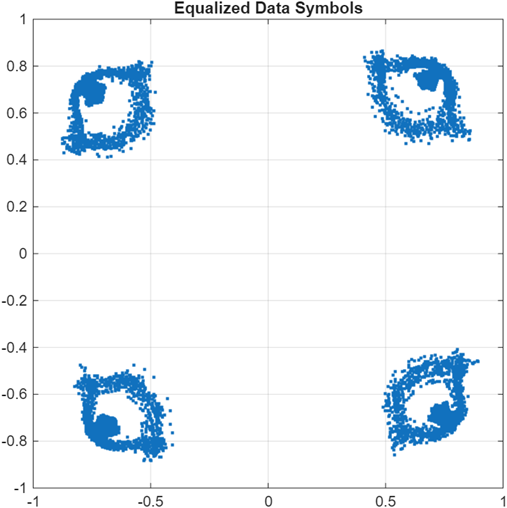
\includegraphics[width=0.3\textwidth]{figures/chap3_channel/c3_3.png} &
        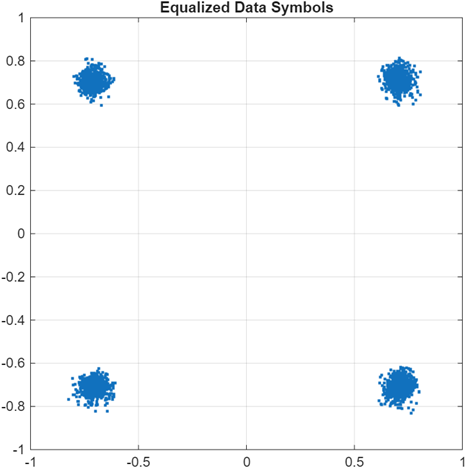
\includegraphics[width=0.3\textwidth]{figures/chap3_channel/c3_4.png} &
        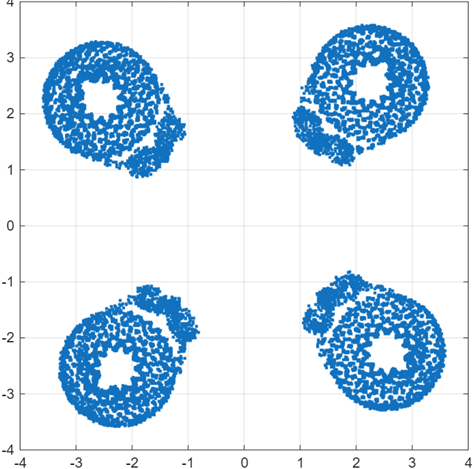
\includegraphics[width=0.3\textwidth]{figures/chap3_channel/c3_5.png} \\
        \small (a) MMSE Equalization & \small (b) LS Equalization & \small (c) No Equalization
    \end{tabular}
    \caption[Comparison of Equalization Techniques]{%
        Constellation comparison: (a) MMSE equalization provides optimal clustering; 
        (b) LS equalization shows higher noise sensitivity; 
        (c) Unequalized signal with a closed eye pattern due to severe ISI.
    }%
    \label{fig:constellation_comparison}%
\end{figure}

Regarding ISI, the numerical metric calculated yields $\gamma_{\text{ISI}} \approx 1.0086$, suggesting channel closure (see \Cref{fig:channel_estimation_summary}).
However, visual inspection of the constellation suggests a much lower effective ISI (approximately 0.5), with clearly separable symbols.
This discrepancy likely arises because the ISI metric is computed from the estimated channel response, which inevitably includes estimation noise, inflating the calculated interference.

\section{Channel 4: Band Rejection} \label{sec:Channel4}

Initial transmission over Channel 4 resulted in a scattered constellation resembling a chaotic cloud, yielding a BER of nearly 0.5.
Analysis of the frequency response reveals a deep spectral notch or band-rejection characteristic, where the magnitude of central subcarriers drops to near zero (see \Cref{fig:ch4_frequency_report}).
Inverting such a channel causes the equalizer to amplify noise infinitely at the nulls (singular matrix problem).

\begin{figure}[!ht]
    \fcapside[\FBwidth]{%
        \captionsetup{parskip = .5\baselineskip plus 1pt}%
        \caption[]{%
             Frequency response analysis revealing a significant band rejection.
        }%
        \label{fig:ch3_freqResp}%
    }{%
        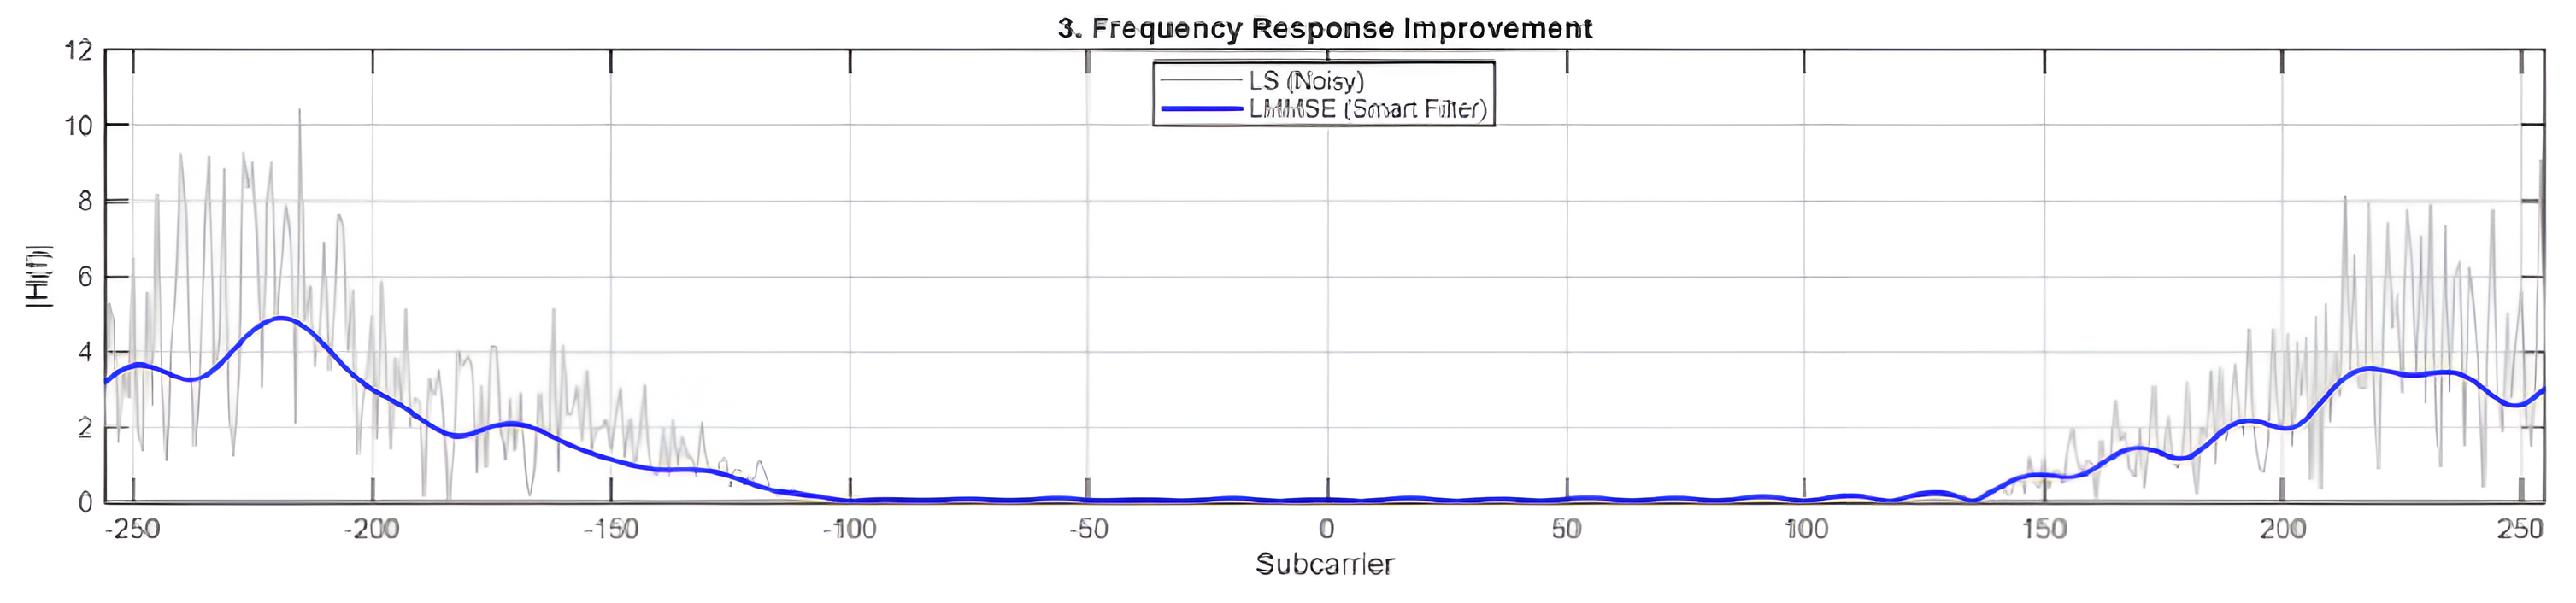
\includegraphics[width=0.70\textwidth]{figures/chap3_channel/c4_7.png}
    }
\end{figure}

To circumvent this, we adopted a sideband transmission strategy, deactivating the subcarriers within the rejection band.
While this necessitated increasing the frame duration to maintain data throughput, it successfully bypassed the deep fade.
As shown in \Cref{fig:ch4_constellations}, this strategy reduced the BER to \num{0.023107}.

\begin{figure}[!ht]
    \centering
    \captionsetup{parskip = .5\baselineskip plus 1pt}
    \begin{tabular}{cc}
        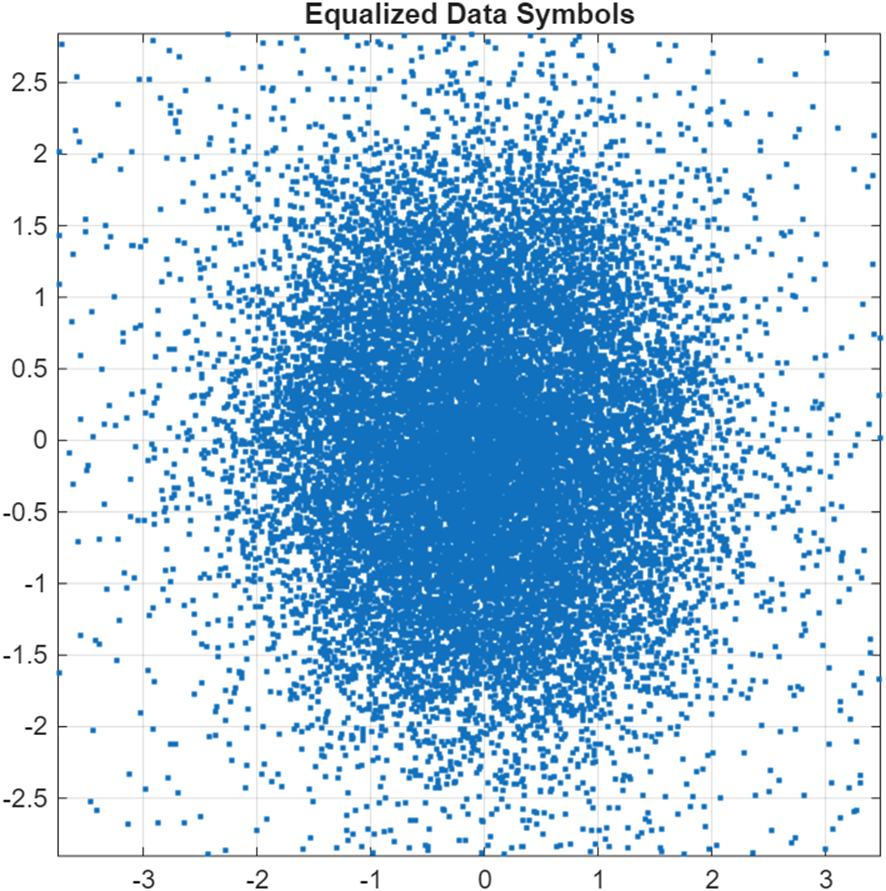
\includegraphics[width=0.45\textwidth]{figures/chap3_channel/c4_1.png} &
        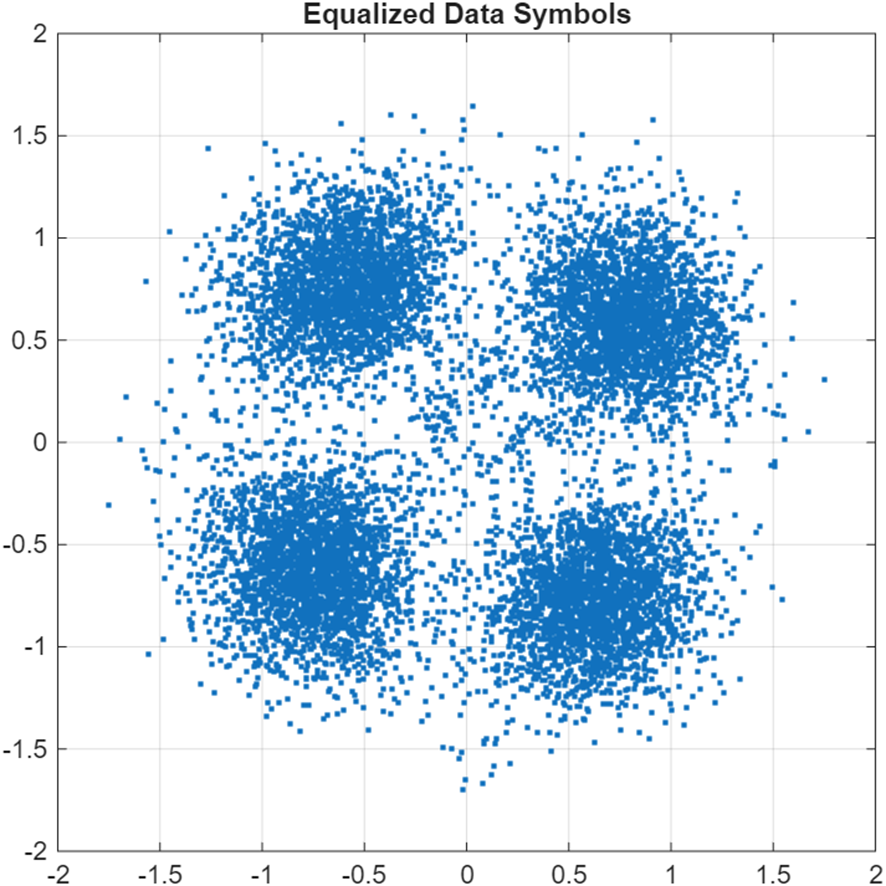
\includegraphics[width=0.45\textwidth]{figures/chap3_channel/c4_3.png} \\
        \small (a) Initial Equalized Symbols & \small (b) Improved Sideband Reception
    \end{tabular}
    \caption[Channel 4: Band-Rejection Equalization Comparison]{%
        Comparison of received 4-QAM constellations for Channel 4: (a) High BER reception due to band-rejection characteristics; 
        (b) Improved constellation achieved by activating sideband subcarriers, leading to lower bit error rates.
    }%
    \label{fig:ch4_constellations}%
\end{figure}

Additionally, \Cref{fig:ch4_correlation} illustrates the signal magnitude and the normalized correlation metric used for frame detection in this band-limited scenario.

\section{Channel 5: Multipath Fading} \label{sec:Channel5}

Channel 5 exhibits the characteristics of a typical multipath environment.
The time-domain view shows a sequence of taps with exponentially decaying amplitudes, representing discrete signal paths with varying delays and attenuations.
The PDP and frequency response are detailed in \Cref{fig:ch5_pdp_analysis} and \Cref{fig:ch5_numerical_summary}.

Consistent with our methodology, the raw LS estimate is noisy.
By applying a window to the impulse response, we obtain a smoothed frequency response that mitigates noise enhancement.
\Cref{fig:ch5_ber_performance} compares the BER performance across different strategies:
\begin{itemize}
    \item \textbf{No Equalization}: Results in a BER of 0.5 (failure).
    \item \textbf{LS Equalization}: Provides functional performance but remains suboptimal due to noise.
    \item \textbf{MMSE (Window $L=15$)}: Yields the best performance, as the window length matches the significant channel taps.
    \item \textbf{MMSE (Window $L=150$)}: Performance degrades and approaches the LS curve, as the wide window admits excessive noise.
\end{itemize}

\begin{figure}[!ht]
    \centering
    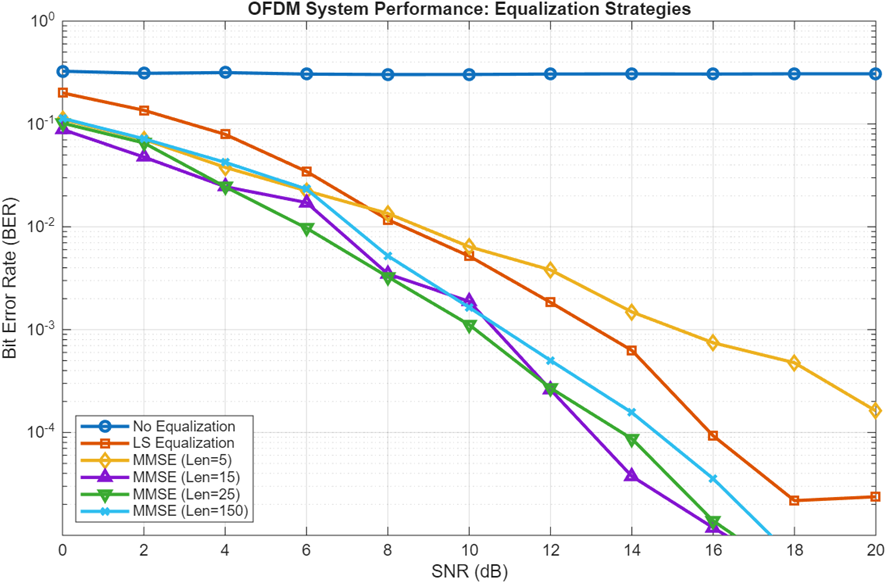
\includegraphics[width=0.85\textwidth]{figures/chap3_channel/c5_2.png}
    \caption[Channel 5: BER Performance Comparison]{%
        Bit Error Rate (BER) performance curves for Channel 5. The plot compares the performance of an unequalized system, LS equalization, and MMSE equalization with varying filter lengths ($L=5, 15, 25, 150$).
    }%
    \label{fig:ch5_ber_performance}%
\end{figure}

For a visual confirmation of the equalization success, the recovered 4-QAM constellation is provided in \Cref{fig:ch5_constellation} in the appendix.


\begin{idea}[Optimization Proposal: Adaptive Cyclic Prefix]
    The Cyclic Prefix (CP) is a critical mechanism to mitigate Inter-Symbol Interference (ISI), yet its standard configuration often incurs unnecessary overhead.
    Per the project specifications, a fixed CP length of $N_{\text{CP}} = 256$ samples is mandated for an OFDM symbol size of $N = 512$ subcarriers. While robust, this results in a significant efficiency loss of approximately $1/3$ of the transmission time.
    
    To address this, we propose an adaptive CP strategy based on the effective Channel Impulse Response (CIR) length.
    Our experimental results confirm that efficiency can be maximized without compromising signal integrity by tailoring the CP to each specific channel:
    \begin{itemize}
        \item \textbf{Channels 1 \& 2 (Flat Fading):} As these channels exhibit negligible delay spread, the CP can be drastically reduced to a single sample (or removed entirely), maximizing data throughput.
        \item \textbf{Channel 5 (Multipath):} A reduced CP of approximately 15 samples suffices to cover the delay spread, significantly lower than the default 256.
        \item \textbf{Channel 3 (High Dispersion):} Due to the severe delay spread, retaining the full CP length is necessary to prevent ISI.
    \end{itemize}
    This tailored approach ensures that the system operates at maximum efficiency for the given physical channel conditions.
\end{idea}